\chapter{Algorytm \textit{L*}}
\label{cha:l-star}

Algorytm \textit{L*} \cite{L_STAR} jest fundamentalnym podejściem do uczenia się języków regularnych za pomocą zapytań i kontrprzykładów. Jego celem jest skonstruowanie minimalnego automatu deterministycznego (DFA), który rozpoznaje dany język regularny, na podstawie ograniczonych interakcji między dwoma uczestnikami procesu uczenia: \textbf{nauczycielem} i \textbf{uczniem}.

\section{Metoda}

Konstruowanie minimalnego automatu deterministycznego (DFA), który akceptuje język \( L \), odbywa się przy pomocy dwóch rodzajów zapytań:
\begin{itemize}
    \item \textbf{Zapytania o członkostwo (Membership Queries, \textit{MQ}):} Uczeń pyta, czy słowo \( w \) należy do języka \( L \). Nauczyciel odpowiada „tak” (\( w \in L \)) lub „nie” (\( w \notin L \)).
    \item \textbf{Zapytania o równoważność (Equivalence Queries, \textit{EQ}):} Uczeń przedstawia hipotezę \( H \), reprezentującą język \( L(H) \), i pyta, czy \( L(H) = L \). Jeśli hipoteza jest niepoprawna, nauczyciel dostarcza kontrprzykład \( w \), dla którego \( w \in L \) i \( w \notin L(H) \), lub \( w \notin L \) i \( w \in L(H) \).
\end{itemize}

Nauczyciela często nazywa się też \textbf{wyrocznią} jako skrót myślowy, ponieważ formalnie nauczyciel jest parą \textbf{wyroczni (oracles)} \textit{MQ} i \textit{EQ}.

Proces algorytmu \textit{L*} opiera się na iteracyjnym konstruowaniu \textbf{tabeli obserwacji (Observation Table)}, która zawiera informacje o języku \( L \) zebrane z zapytań \textit{MQ}. Na podstawie tabeli tworzone są kolejne hipotezy automatu DFA, które są następnie testowane za pomocą zapytań \textit{EQ}.

Główne kroki algorytmu:
\begin{enumerate}
    \item \textbf{Inicjalizacja:} Algorytm rozpoczyna od utworzenia tabeli obserwacji z minimalnymi zbiorami prefiksów (\( S \)) i sufiksów (\( E \)).
    \item \textbf{Sprawdzanie zamknięcia i spójności:} Algorytm weryfikuje, czy tabela obserwacji spełnia wymagania:
    \begin{itemize}
        \item \textbf{Zamknięcie:} Każdy prefiks prowadzi do jednego ze znanych stanów.
        \item \textbf{Spójność:} Wiersze tabeli są rozróżnialne za pomocą sufiksów w \( E \).
    \end{itemize}
    \item \textbf{Tworzenie hipotezy:} Na podstawie tabeli obserwacji generowany jest automat DFA \( H \).
    \item \textbf{Test równoważności:} Hipoteza \( H \) jest testowana za pomocą \textit{EQ}. W przypadku błędu tabela jest aktualizowana na podstawie kontrprzykładu.
    \item \textbf{Terminacja:} Proces kończy się, gdy hipoteza \( H \) jest poprawna.
\end{enumerate}

\section{Formalizacja}

\subsection{Języki regularne i automaty deterministyczne (DFA)}

Niech \( L \subseteq \Sigma^* \) będzie językiem regularnym zdefiniowanym nad alfabetem \( \Sigma \). Język \( L \) jest akceptowany przez automat deterministyczny (DFA) \( M = (Q, \Sigma, \delta, q_0, F) \), gdzie:
\begin{itemize}
    \item \( Q \): skończony zbiór stanów,
    \item \( \Sigma \): alfabet,
    \item \( \delta: Q \times \Sigma \to Q \): funkcja przejścia,
    \item \( q_0 \in Q \): stan początkowy,
    \item \( F \subseteq Q \): zbiór stanów akceptujących.
\end{itemize}

Automat \( M \) akceptuje słowo \( w \in \Sigma^* \), jeśli \( \delta(q_0, w) \in F \), gdzie \( \delta(q_0, w) \) oznacza iteracyjne zastosowanie \( \delta \) do \( w \).

\subsection{Tabela obserwacji}

Tabela obserwacji \( ObservationTable \) to struktura danych definiowana jako \( (S, E, T) \), gdzie:
\begin{itemize}
    \item \( S \subseteq \Sigma^* \): skończony zbiór prefiksów,
    \item \( E \subseteq \Sigma^* \): skończony zbiór sufiksów,
    \item \( T: (S \cup S \cdot \Sigma) \times E \to \{0, 1\} \): funkcja wartościująca wynik zapytania \( MQ(s \cdot e) \), gdzie \( s \in S \cup S \cdot \Sigma \) i \( e \in E \).
\end{itemize}

\subsection{Warunki poprawności tabeli obserwacji}

Tabela obserwacji \( ObservationTable \) musi spełniać dwa warunki:
\begin{enumerate}
    \item \textbf{Zamknięcie:} Dla każdego \( s \in S \cdot \Sigma \), istnieje \( s' \in S \), taki że \( \forall e \in E, \, T(s, e) = T(s', e) \).
    \item \textbf{Spójność:} Dla wszystkich \( s_1, s_2 \in S \), jeśli \( \forall e \in E, \, T(s_1, e) = T(s_2, e) \), to dla każdego \( a \in \Sigma \), \( \forall e \in E, \, T(s_1 \cdot a, e) = T(s_2 \cdot a, e) \).
\end{enumerate}

\subsection{Tworzenie hipotezy}

Na podstawie tabeli \( ObservationTable \), która spełnia warunki zamknięcia i spójności, można skonstruować DFA \( H = (Q, \Sigma, \delta, q_0, F) \), gdzie:
\begin{itemize}
    \item \( Q = \{[s] \mid s \in S\} \), gdzie \( [s] \) oznacza klasę równoważności \( s \) w \( T \),
    \item \( \delta([s], a) = [s \cdot a] \),
    \item \( q_0 = [\epsilon] \),
    \item \( F = \{[s] \mid T(s, \epsilon) = 1\} \).
\end{itemize}

\subsection{Kontrprzykłady i aktualizacja tabeli}

Jeśli hipoteza \( H \) nie jest równoważna \( L \), Nauczyciel dostarcza kontrprzykład \( w \). Prefiksy \( w \) są dodawane do \( S \), a tabela jest aktualizowana zgodnie z wynikami zapytań \( MQ \).

\section{Złożoność czasowa}

Algorytm \textit{L*} składa się z kilku etapów, których złożoność można szczegółowo przeanalizować. Złożoność czasowa jest wielomianowa, co zostało wykazane \cite{L_STAR}.

\section{Złożoność pamięciowa}

Przyjmijmy:
\begin{itemize}
    \item \(n\) - liczba stanów szukanego minimalnego DFA,
    \item \(m\) - maksymalna długość kontrprzykładu,
    \item \(|\Sigma|\) - rozmiar alfabetu.
\end{itemize}

\subsubsection*{Struktura danych}
\begin{itemize}
    \item \textbf{Tabela obserwacji:}
    \begin{itemize}
        \item Zbiór \(S\) (prefiksy): maksymalnie \(O(n + m \cdot (n - 1))\) wpisów,
        \item Zbiór \(E\) (sufiksy): maksymalnie \(O(n)\) wpisów,
        \item Całkowity rozmiar tabeli: \(O(n \cdot m)\).
    \end{itemize}
    \item \textbf{DFA hipotezy:}
    \begin{itemize}
        \item DFA może mieć maksymalnie \(n\) stanów i \(O(n \cdot |\Sigma|)\) przejść.
    \end{itemize}
\end{itemize}

\subsubsection*{Łączna złożoność pamięciowa}
Algorytm wymaga pamięci na tabelę obserwacji oraz strukturę DFA:
\[
O(n \cdot m + n \cdot |\Sigma|).
\]

Podsumowując czynnikami wpływającymi na złożoność są:
\begin{itemize}
    \item \textbf{Rozmiar alfabetu (\(|\Sigma|\))}: Większy alfabet oznacza więcej przejść w tabeli obserwacji i DFA.
    \item \textbf{Długość kontrprzykładów (\(m\))}: Dłuższe kontrprzykłady zwiększają liczbę zapytań o członkostwo i rozmiar tabeli obserwacji.
    \item \textbf{Liczba stanów DFA (\(n\))}: Więcej stanów oznacza większą tabelę obserwacji i więcej iteracji algorytmu.
\end{itemize}

\section{Przykład działania}

Aby rozjaśnić działanie algorytmu \textit{L*}, rozważmy prosty język \( L \)

\[
L = \{w \in \{a, b\}^* \mid \text{liczba liter } a \text{ w } w \text{ jest parzysta}\}.
\]

Minimalny DFA dla tego języka można zobaczyć na rysunku \ref{fig:dfa_even_a}. Automat ten ma dwa stany:
\begin{itemize}
    \item Stan \( s_0 \): parzysta liczba \( a \),
    \item Stan \( s_1 \): nieparzysta liczba \( a \).
\end{itemize}

\begin{figure}[ht]
    \centering
    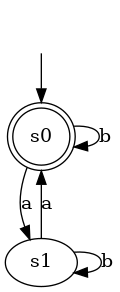
\includegraphics[width=0.2\linewidth]{images/dfa_even_a.png}
    \caption{Minimalny DFA generujący język \textit{L}.}
    \label{fig:dfa_even_a}
\end{figure}

\subsection*{Kroki algorytmu}

\paragraph*{Inicjalizacja tabeli obserwacji.}
Rozpoczynamy od tworzenia minimalnych zbiorów \textit{S} i \textit{E}:
\[
S = \{\epsilon\}, \quad E = \{\epsilon\}.
\]
Uczeń zadaje zapytanie o członkostwo \( MQ(\epsilon) \), a Nauczyciel odpowiada „tak”, ponieważ \( \epsilon \in L \). Na tej podstawie tabela obserwacji wygląda następująco (warto odnotować, że przykład jest na tyle prosty, że nie zwiększymy zbioru \textit{E}, w przeciwnym wypadku powstałoby więcej kolumn):

\[
\begin{array}{c|c}
S \cup (S \cdot \Sigma) \setminus E & \epsilon \\
\hline
\epsilon      & 1 \\
\end{array}
\]

\paragraph*{Dodanie nowych wierszy.}
Uczeń dodaje \( S \cdot \Sigma = \{a, b\} \) do tabeli i zadaje zapytania o członkostwo:
\[
MQ(a) = 0, \quad MQ(b) = 1.
\]
Aktualizacja tabeli:

\[
\begin{array}{c|c}
S \cup (S \cdot \Sigma) \setminus E & \epsilon \\
\hline
\epsilon      & 1 \\
\hline
a             & 0 \\
b             & 1 \\
\end{array}
\]

Tabela jest \textbf{niezamknięta}, ponieważ dla \(a\) nie istnieje takie \(s\), że \( \forall e \in E, \, T(a, e) = T(s, e) \).

\paragraph*{Rozszerzenie \( S \).}
Dodajemy \( a \) do \( S \), aby tabela była zamknięta:
\[
S = \{\epsilon, a\}.
\]

Nowa tabela obserwacji:
\[
\begin{array}{c|c}
S \cup (S \cdot \Sigma) \setminus E & \epsilon \\
\hline
\epsilon      & 1 \\
a             & 0 \\
\hline
b             & 1 \\
aa            & 1 \\
ab            & 0 \\
\end{array}
\]

Tabela jest teraz \textbf{zamknięta}. Jest też ona spójna. Możemy teraz skonstruować hipotezę.

\paragraph*{Konstrukcja hipotezy automatu.}
Na podstawie tabeli obserwacji konstruujemy hipotezę automatu DFA:
\begin{itemize}
    \item \textbf{Stany DFA:} \( q_\epsilon, q_a \), odpowiadające \( T(\epsilon, \epsilon) \) oraz \( T(a, \epsilon) \).
    \item \textbf{Przejścia:}
    \begin{align*}
        & q_\epsilon \xrightarrow{a} q_a, \quad q_\epsilon \xrightarrow{b} q_\epsilon, \\
        & q_a \xrightarrow{a} q_\epsilon, \quad q_a \xrightarrow{b} q_a.
    \end{align*}
    \item \textbf{Stan początkowy:} \( q_\epsilon \), ponieważ odpowiada wierszowi \( \epsilon \).
    \item \textbf{Stany akceptujące:} \( q_\epsilon \), ponieważ odpowiada \( T(\epsilon, \epsilon) = 1 \).
    \item \textbf{Stany nieakceptujące:} \( q_a \), ponieważ \( T(a, \epsilon) = 0 \).
\end{itemize}

\paragraph*{Testowanie hipotezy.}
Hipoteza jest testowana przez zapytanie o równoważność (EQ). Nauczyciel odpowiada "tak" co kończy działanie algorytmu. 

\paragraph*{Ostateczny automat.}
Automat DFA reprezentujący język o parzystej liczbie \( a \):
\[
\begin{array}{c|c|c}
\text{Stan} & a & b \\
\hline
\rightarrow * q_\epsilon & q_a & q_\epsilon \\
q_a & q_\epsilon & q_a \\
\end{array}
\]

% Opcjonalnie zastosowania i rozszerzenia
